\documentclass[11pt, compress, aspectratio=1610]{beamer}
% Set language
\usepackage{xstring}
\newcommand{\Langue}[1]{%
    \IfEqCase{#1}{%
        {francais}{
        \usepackage[utf8]{inputenc}
        \usepackage[francais]{babel}
        }%
        {english}{\usepackage[english]{babel}}%
    }[\PackageError{Langue}{Undefined option to language: #1}{}]%
}%
\Langue{francais}

\usetheme{pl}
\usepackage{tikz}
  \usetikzlibrary{arrows, plotmarks, decorations.markings}
  \tikzstyle{fleche} = [->,>=stealth,thick,rounded corners=4pt,line width=0.7pt]
  \tikzstyle{fleche2} = [->,>=stealth,thick,dashed,rounded corners=4pt,line width=1pt]
  \tikzstyle{fleche3} = [->,>=stealth,thick,rounded corners=4pt,line width=4pt]
  \tikzstyle{fleche4} = [->,>=stealth,thick,dashed,rounded corners=4pt,line width=0.5pt]
  \tikzstyle{fleche5} = [->,>=stealth,thick,rounded corners=4pt,line width=2pt]
  \usetikzlibrary{shadows}
  \usetikzlibrary{shadings,decorations.pathreplacing,angles,quotes,overlay-beamer-styles}
  \usetikzlibrary{positioning}
  \tikzstyle{trait} = [-,>=stealth,rounded corners=2pt,line width=0.7pt]
  \usetikzlibrary{automata,shapes.multipart}
 \usepackage{relsize}
\usepackage{longtable}
\usepackage{booktabs}
\usepackage{minted}
\usepackage{listings}
\usepackage{color}
\usepackage{fancyvrb}
\newcommand{\VerbBar}{|}
\newcommand{\VERB}{\Verb[commandchars=\\\{\}]}
\DefineVerbatimEnvironment{Highlighting}{Verbatim}{commandchars=\\\{\},fontsize=\small}
% Add ',fontsize=\small' for more characters per line
\usepackage[framemethod=tikz]{mdframed}
\definecolor{shadecolor}{HTML}{EEEEEE}
\mdfsetup{
  backgroundcolor=shadecolor,
  linecolor=shadecolor,
  innerleftmargin=5pt,
  innerrightmargin=5pt,
  leftmargin=-5pt,
  rightmargin=-5pt,
  roundcorner=3pt
}
\newenvironment{Shaded}{\begin{mdframed}}{\end{mdframed}}
\newcommand{\KeywordTok}[1]{\textcolor[rgb]{0.26,0.66,0.93}{\textbf{{#1}}}}
\newcommand{\DataTypeTok}[1]{\textcolor[rgb]{0.74,0.68,0.62}{\underline{{#1}}}}
\newcommand{\DecValTok}[1]{\textcolor[HTML]{558B2F}{{#1}}}
\newcommand{\BaseNTok}[1]{\textcolor[HTML]{558B2F}{{#1}}}
\newcommand{\FloatTok}[1]{\textcolor[HTML]{558B2F}{{#1}}}
\newcommand{\ConstantTok}[1]{\textcolor[rgb]{0.74,0.68,0.62}{{#1}}}
\newcommand{\CharTok}[1]{\textcolor[HTML]{7E57C2}{{#1}}}
\newcommand{\SpecialCharTok}[1]{\textcolor[HTML]{7E57C2}{{#1}}}
\newcommand{\StringTok}[1]{\textcolor[HTML]{7E57C2}{{#1}}}
\newcommand{\VerbatimStringTok}[1]{\textcolor[HTML]{7E57C2}{{#1}}}
\newcommand{\SpecialStringTok}[1]{\textcolor[HTML]{7E57C2}{{#1}}}
\newcommand{\ImportTok}[1]{\textcolor[rgb]{0.74,0.68,0.62}{{#1}}}
\newcommand{\CommentTok}[1]{\textcolor[HTML]{546E7A}{\textit{{#1}}}}
\newcommand{\DocumentationTok}[1]{\textcolor[HTML]{BCAAA4}{\textit{{#1}}}}
\newcommand{\AnnotationTok}[1]{\textcolor[HTML]{BCAAA4}{\textbf{\textit{{#1}}}}}
\newcommand{\CommentVarTok}[1]{\textcolor[rgb]{0.74,0.68,0.62}{{#1}}}
\newcommand{\OtherTok}[1]{\textcolor[rgb]{0.74,0.68,0.62}{{#1}}}
\newcommand{\FunctionTok}[1]{\textcolor[HTML]{26A69A}{\textbf{{#1}}}}
\newcommand{\VariableTok}[1]{\textcolor[rgb]{0.74,0.68,0.62}{{#1}}}
\newcommand{\ControlFlowTok}[1]{\textcolor[rgb]{0.26,0.66,0.93}{\textbf{{#1}}}}
\newcommand{\OperatorTok}[1]{\textcolor[rgb]{0.74,0.68,0.62}{{#1}}}
\newcommand{\BuiltInTok}[1]{\textcolor[HTML]{42A5F5}{{#1}}}
\newcommand{\ExtensionTok}[1]{\textcolor[rgb]{0.74,0.68,0.62}{{#1}}}
\newcommand{\PreprocessorTok}[1]{\textcolor[rgb]{0.74,0.68,0.62}{\textbf{{#1}}}}
\newcommand{\AttributeTok}[1]{\textcolor[rgb]{0.74,0.68,0.62}{{#1}}}
\newcommand{\RegionMarkerTok}[1]{\textcolor[rgb]{0.74,0.68,0.62}{{#1}}}
\newcommand{\InformationTok}[1]{\textcolor[rgb]{0.00,0.40,1.00}{\textbf{\textit{{#1}}}}}
\newcommand{\WarningTok}[1]{\textcolor[HTML]{FF6E40}{\textbf{{#1}}}}
\newcommand{\AlertTok}[1]{\textcolor[HTML]{FF3D00}{{#1}}}
\newcommand{\ErrorTok}[1]{\textcolor[HTML]{DD2C00}{\textbf{{#1}}}}
\newcommand{\NormalTok}[1]{\textcolor[HTML]{212121}{{#1}}}
\newcommand\smallcitation[1]{% command to add small citation in the corner
\begin{textblock*}{\textwidth}(30pt,\textheight)
    \raggedleft \small\textit{#1}
\end{textblock*}}
\providecommand{\tightlist}{%
  \setlength{\itemsep}{0pt}\setlength{\parskip}{0pt}}

\let\OldTexttt\texttt
\renewcommand{\texttt}[1]{\OldTexttt{\color{plTT}#1}}

\makeatletter
\def\maxwidth{\ifdim\Gin@nat@width>\linewidth\linewidth\else\Gin@nat@width\fi}
\makeatother

\usepgfplotslibrary{dateplot}

\newcommand{\begincols}{\begin{columns}}
\newcommand{\stopcols}{\end{columns}}
\newcommand{\roundpicture}[2]{%
\tikz\node[circle,
          text=white,
          minimum width=4cm,
          minimum height=4cm,
          path picture={
              \node at (path picture bounding box.center){
                  \includegraphics[width=4cm]{#1}
              };
          }]{#2};
}
\newcommand{\plain}[1]{%
\begin{picture}(0,0)
  \put(-28.5,-175){%
      \pgfuseimage{titlebackground}
  }
  \put(0,-145){%
      \begin{minipage}[b][4.5cm][t]{0.5\textwidth}
          \color{white}\huge
              #1
      \end{minipage}
  }
\end{picture}
}

\title{Effets de la température sur la régulation trophique}
\subtitle{Séminaire 1}
\date{\today}
\author{\textbf{Azenor Bideault}\\
Superviseurs: Dominique Gravel \& Michel Loreau \newline}
\institute{Université de Sherbooke}

\begin{document}

\maketitle

\begin{frame}{Température: gradient environnemental majeur}

\centering
Température annuelle moyenne
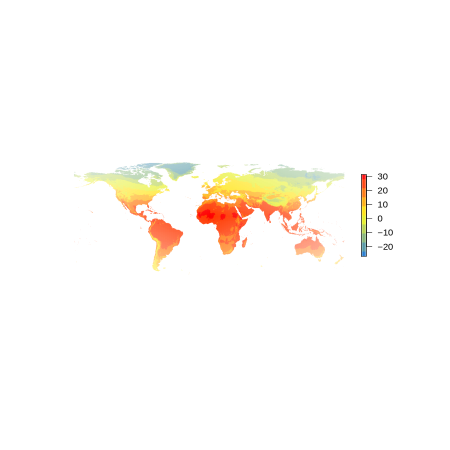
\includegraphics[width=1\linewidth]{figuresAz/AnmeanTempST.pdf}
\smallcitation{Données de Worldclim}

\end{frame}

\begin{frame}{Effets de la température}

\begincols
 \column{0.48\textwidth} \centering
 Taux métabolique \par
 \includegraphics[width=0.4\linewidth]{figuresAz/cell.png}\par
 \vspace{1cm} \pause
 Taux biologiques (taux de croissance) \par
 
\includegraphics[width=0.5\linewidth]{figuresAz/fish_pop.pdf} \pause
 \hfill\column{0.48\textwidth} \centering
 Taille corporelle \par
 \includegraphics[width=0.6\linewidth]{figuresAz/size.pdf}\par
 \vspace{1cm} \pause
 Distribution des espèces \par
 \includegraphics[width=0.8\linewidth]{figuresAz/world.pdf} \par

\stopcols

\end{frame}

\begin{frame}{Effets des interactions trophiques à l'échelle du paysage}

\centering
 \includegraphics[width=0.7\linewidth]{figuresAz/estes2011.png}\par
\smallcitation{Estes \textit{et al} 2011}

\end{frame}

\begin{frame}{Effets de la température sur la régulation trophique}

\centering
 \input{figuresAz/schema2.tex}\par

\end{frame}

\begin{frame}{Effets de la température sur la régulation trophique}

\centering
% \documentclass[12pt,a4paper]{article}
%
% %%%%%%%%%%%%%%%%%%%%%%%%%%
% %% Packages %%
% % font
% \usepackage[T1]{fontenc}
% \usepackage[utf8]{inputenc}
% % language
% \usepackage[french, english]{babel}
%
% % marges, space...
% \usepackage[top=2.5cm, bottom=2.5cm, left=2.5cm, right=2.5cm]{geometry}
% \usepackage{setspace}
% \onehalfspacing
% \usepackage[font=footnotesize,labelfont=bf]{caption}
% \usepackage{subcaption}
%
% \usepackage{graphicx}
% \usepackage{float}
% \usepackage{pstool}
% \usepackage{multirow}
% \usepackage{booktabs,arydshln}
% % mathematics
% \usepackage{amsmath}
% \usepackage{textcomp}
%
% % TikZ
% \usepackage{tikz}
% 	\usetikzlibrary{arrows, plotmarks, decorations.markings}
% 	\tikzstyle{fleche} = [->,>=stealth,thick,rounded corners=4pt,line width=1pt]
% 	\tikzstyle{fleche2} = [->,>=stealth,thick,dashed,rounded corners=4pt,line width=2pt]
% 	\tikzstyle{fleche3} = [->,>=stealth,thick,rounded corners=4pt,line width=2pt]
% 	\usetikzlibrary{shadows}
% 	\usetikzlibrary{shadings,decorations.pathreplacing,angles,quotes}
%
%
% %%%%%%%%%%%%%%%%%%%%%%%%%%
%
% \begin{document}

%
% % FIGURE MODEL %%
% \begin{figure}[!h]


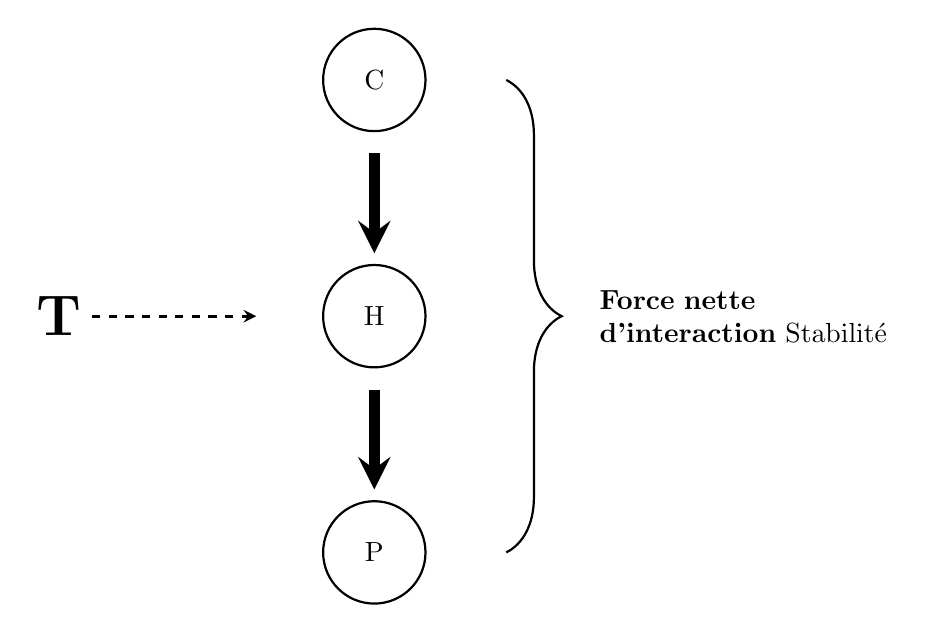
\begin{tikzpicture}[thick]
	\draw (4,6) circle (0.65);
	\node (C) at (4,6) {C};

	\draw (4,3) circle (0.65);
	\node (H) at (4,3) {H};

	\draw (4,0) circle (0.65);
	\node (P) at (4,0) {P};

	\node (T) at (0,3) {\textbf{\huge T}};

	\node (CH) at (4,5.2) {};
	\draw[fleche3] (CH) -- (4,3.8);

	\node (HP) at (4,2.2) {};
	\draw[fleche3] (HP) -- (4,0.8);

	\draw[fleche2]	(T) to node [midway] (H) {} (2.5,3);


\draw[decoration={brace,mirror,raise=5pt,amplitude=20pt},decorate]
	  (5.5,0) -- node[right=35pt, text width = 4cm] (FI) {\textbf{Force nette d'interaction}  Stabilité} (5.5,6);

\end{tikzpicture}
% \end{figure}
%
% \end{document}
\par
\smallcitation{Beveridge et al 2010, Kratina et al 2012, Shurin et al 2012}

\end{frame}

\begin{frame}{Effets de la température sur la régulation trophique}

\input{figuresAz/schemaSC.tex}\par
\smallcitation{Vasseur \& McCann 2005, Brose et al 2012, Fussman et al 2014}

\end{frame}

\begin{frame}{Force nette d'interaction}

\centering
% \documentclass[12pt,a4paper]{article}
%
% %%%%%%%%%%%%%%%%%%%%%%%%%%
% %% Packages %%
% % font
% \usepackage[T1]{fontenc}
% \usepackage[utf8]{inputenc}
% % language
% \usepackage[french, english]{babel}
%
% % marges, space...
% \usepackage[top=2.5cm, bottom=2.5cm, left=2.5cm, right=2.5cm]{geometry}
% \usepackage{setspace}
% \onehalfspacing
% \usepackage[font=footnotesize,labelfont=bf]{caption}
% \usepackage{subcaption}
%
% \usepackage{graphicx}
% \usepackage{float}
% \usepackage{pstool}
% \usepackage{multirow}
% \usepackage{booktabs,arydshln}
% % mathematics
% \usepackage{amsmath}
% \usepackage{textcomp}
%
% % TikZ
% \usepackage{tikz}
% 	\usetikzlibrary{arrows, plotmarks, decorations.markings}
% 	\tikzstyle{fleche} = [->,>=stealth,thick,rounded corners=4pt,line width=1pt]
% 	\tikzstyle{fleche2} = [->,>=stealth,thick,dashed,rounded corners=4pt,line width=2pt]
% 	\tikzstyle{fleche3} = [->,>=stealth,thick,rounded corners=4pt,line width=2pt]
% 	\usetikzlibrary{shadows}
% 	\usetikzlibrary{shadings,decorations.pathreplacing,angles,quotes}
%
%
% %%%%%%%%%%%%%%%%%%%%%%%%%%
%
% \begin{document}
%
%
% % FIGURE MODEL %%
% \begin{figure}[!h]


\begin{tikzpicture}[thick]
	\draw (6,3) circle (0.65);
	\node (H) at (6,3) {H};

	\draw (6,0) circle (0.65);
	\node (PH) at (6,0) {$P_H$};

	\draw (4,0) circle (0.65);
	\node (P0) at (4,0) {$P_0$};

	\node (lPH) at (6,2.2) {};
	\draw[fleche] (lPH) -- (6,0.8);

\draw[decoration={brace,mirror,raise=5pt,amplitude=20pt},decorate]
	  (3,-1) -- node[below=35pt] (D) {Ratio de densité $\dfrac{P_0}{P_H}$} (7,-1);

\end{tikzpicture}
% \end{figure}
%
% \end{document}
\par

\end{frame}

\begin{frame}{Stabilité: taux de retour à l'équilibre}

\begincols
\column{0.48\textwidth}

\centering
\includegraphics[width=1\linewidth]{figuresAz/stab.pdf}

\hfill\column{0.48\textwidth}

\begin{itemize}
\tightlist
\item
  Perturbations ponctuelles: épidémies, feux, inondations\ldots{}
\item
  Taux de retour \(\tau\)
\end{itemize}

\stopcols

\end{frame}

\begin{frame}{Objectif}

\centering
\Large{\textcolor{plST}{Comprendre de façon méchanistique les effets de la température sur la régulation trophique et la structure des réseaux afin de formaliser la théorie}}
\par

\large{En combinant des approches théoriques et expérimentales}

\end{frame}

\begin{frame}{Relation régulation trophique - température}

\input{figuresAz/schemaChap.tex}

\end{frame}

\section{\texorpdfstring{Tester expérimentalement la \mbox{théorie:}
relation température - régulation
trophique}{Tester expérimentalement la  relation température - régulation trophique}}\label{tester-expuxe9rimentalement-la-relation-tempuxe9rature---ruxe9gulation-trophique}

\begin{frame}{Approche quantitative}

\centering
\input{figuresAz/schema_phd1.tex}\par

\end{frame}

\begin{frame}{Approche quantitative}

\centering
% \documentclass[12pt,a4paper]{article}
%
% %%%%%%%%%%%%%%%%%%%%%%%%%%
% %% Packages %%
% % font
% \usepackage[T1]{fontenc}
% \usepackage[utf8]{inputenc}
% % language
% \usepackage[french, english]{babel}
%
% % marges, space...
% \usepackage[top=2.5cm, bottom=2.5cm, left=2.5cm, right=2.5cm]{geometry}
% \usepackage{setspace}
% \onehalfspacing
% \usepackage[font=footnotesize,labelfont=bf]{caption}
% \usepackage{subcaption}
%
% \usepackage{graphicx}
% \usepackage{float}
% \usepackage{pstool}
% \usepackage{multirow}
% \usepackage{booktabs,arydshln}
% % mathematics
% \usepackage{amsmath}
% \usepackage{textcomp}
%
% % TikZ
% \usepackage{tikz}
% 	\usetikzlibrary{arrows, plotmarks, decorations.markings}
% 	\tikzstyle{fleche} = [->,>=stealth,thick,rounded corners=4pt,line width=1pt]
% 	\tikzstyle{fleche2} = [->,>=stealth,thick,dashed,rounded corners=4pt,line width=1pt]
% 	\tikzstyle{fleche3} = [->,>=stealth,thick,rounded corners=4pt,line width=2pt]
% 	\usetikzlibrary{shadows}
% 	\usetikzlibrary{shadings,decorations.pathreplacing,angles,quotes}
%
% %
% % %%%%%%%%%%%%%%%%%%%%%%%%%%
% %
%
% \begin{document}
%
%
% %% FIGURE MODEL %%
% \begin{figure}[!h]
% \centering
\begin{tikzpicture}[thick]
%% Texts and rectangles
	\node (Exp) at (4,8) {Expérimentations};

	\node (Para) at (6,6) {Paramètres};

	\node (MM) at (6,4) {\textcolor{plST}{\Large Modèle mathématique}};


	\node (FI) at (4,2) {\textcolor{plST}{\textbf{\Large Force nette d'interaction}}}; % modèle mathématiques
	\node (Stab) at (4,1.6) {\textbf{Stabilité}};


	%% Fleches

	\draw[fleche]	(Exp) -- (Para);
	\draw[fleche]	(Para) -- (MM);
	\draw[fleche5]	(MM) -- (FI);


	\draw[fleche] (Exp) to[out = -135, in = 135] (FI); % nearEnd6 to stay coherent with m6, p6


\end{tikzpicture}
% %
% \end{figure}
%
% \end{document}
\par

\end{frame}

\begin{frame}{La température impacte les taux biologiques des
organismes}

\centering
% \documentclass[12pt,a4paper]{article}
%
% %%%%%%%%%%%%%%%%%%%%%%%%%%
% %% Packages %%
% % font
% \usepackage[T1]{fontenc}
% \usepackage[utf8]{inputenc}
% % language
% \usepackage[french, english]{babel}
%
% % marges, space...
% \usepackage[top=2.5cm, bottom=2.5cm, left=2.5cm, right=2.5cm]{geometry}
% \usepackage{setspace}
% \onehalfspacing
% \usepackage[font=footnotesize,labelfont=bf]{caption}
% \usepackage{subcaption}
%
% \usepackage{graphicx}
% \usepackage{float}
% \usepackage{pstool}
% \usepackage{multirow}
% \usepackage{booktabs,arydshln}
% % mathematics
% \usepackage{amsmath}
% \usepackage{textcomp}
%
% % TikZ
% \usepackage{tikz}
% 	\usetikzlibrary{arrows, plotmarks, decorations.markings}
% 	\tikzstyle{fleche} = [->,>=stealth,thick,rounded corners=4pt,line width=1pt]
% 	\tikzstyle{fleche2} = [->,>=stealth,thick,dashed,rounded corners=4pt,line width=2pt]
% 	\tikzstyle{fleche3} = [->,>=stealth,thick,rounded corners=4pt,line width=2pt]
% 	\usetikzlibrary{shadows}
% 	\usetikzlibrary{shadings,decorations.pathreplacing,angles,quotes}
%
%
% %%%%%%%%%%%%%%%%%%%%%%%%%%
%
% \begin{document}

%
% % FIGURE MODEL %%
% \begin{figure}[!h]


\begin{tikzpicture}[thick]

	\node (mod) at (4,7.5) {Modèle};

	\draw (4,6.5) circle (0.65);
	\node (C) at (4,6.5) {C};

	\draw (4,4) circle (0.65);
	\node (H) at (4,4) {H};

	\draw (4,1.5) circle (0.65);
	\node (P) at (4,1.5) {P};

	\node (T) at (0,4) {\textbf{\huge T}};

	\node (CH) at (4,5.7) {};
	\draw[fleche] (CH) -- (4,4.8);

	\node (HP) at (4,3.2) {};
	\draw[fleche] (HP) -- (4,2.3);

	\draw[fleche2]	(T) to node [midway] (C) {} (2.5,6.5);
	\draw[fleche2]	(T) to node [midway] (H) {} (2.5,4);
	\draw[fleche2]	(T) to node [midway] (P) {} (2.5,1.5);



\draw[decoration={brace,mirror,raise=5pt,amplitude=20pt},decorate]
	  (5.5,1.5) -- node[right=35pt, text width = 4cm] (FI) {Force nette d'interaction} (5.5,6.5);

\end{tikzpicture}
% \end{figure}
%
% \end{document}


\end{frame}

\begin{frame}{Effet de la température sur les taux biologiques}

\begincols
\column{0.48\textwidth}

\centering
\includegraphics[width=1\linewidth]{figuresAz/MTE.pdf}

\hfill\column{0.48\textwidth}

\[
    r(T)= r_0 \textbf{m}^{\beta} exp^{\biggl(-\dfrac{\textbf{E}}{k\textbf{T}}\biggr)}\mathlarger{L}(T)
\]

~

\begin{description}
\tightlist
\item[\(r(T)\)]
taux biologique
\item[\(m\)]
masse corporelle
\item[\(E\)]
énergie d'activation
\item[\(T\)]
température
\item[\(L(T)\)]
phase décroissante
\item[\(\beta\), \(r_0\), \(k\)]
constantes
\end{description}

\stopcols
\smallcitation{Gillooly et al 2001, Brown et al 2004, Savage et al 2004, Pawar et al 2015}

\end{frame}

\begin{frame}{La force nette d'interaction suit la même relation
unimodale}

\begincols
 \column{.48\textwidth} \centering
\input{figuresAz/schema_ITbisSansTextBracket.tex} \column{.48\textwidth}
\centering  \includegraphics[width=1\linewidth]{figuresAz/NetIS.pdf}

\stopcols

\end{frame}

\begin{frame}{Tester expérimentalement la théorie}

\centering
\input{figuresAz/schema_phd1.tex}\par

\end{frame}

\begin{frame}{Modèle d'étude: Interactions bactéries-protistes}

\begincols
\column{0.48\textwidth}

\centering  \includegraphics[width=0.7\linewidth]{figuresAz/pitcher.jpg}

\hfill\column{0.48\textwidth}

\begin{itemize}
\tightlist
\item
  Sarracénies pourpres (\textit{Sarracenia purpurea})
\item
  Protistes-Bactéries
\item
  Expériences en microcosmes
\item
  5 souches de bactéries, 3 espèces de protistes
\item
  Gradient de températures (10-40\(^\circ\)C )
\end{itemize}

\stopcols

\end{frame}

\begin{frame}{Méthode: Cinétique des bactéries et réponse fonctionnelle
des protistes}

\begincols
 \column{.5\textwidth} \centering
 % \documentclass[12pt,a4paper]{article}
%
% %%%%%%%%%%%%%%%%%%%%%%%%%%
% %% Packages %%
% % font
% \usepackage[T1]{fontenc}
% \usepackage[utf8]{inputenc}
% % language
% \usepackage[french, english]{babel}
%
% % marges, space...
% \usepackage[top=2.5cm, bottom=2.5cm, left=2.5cm, right=2.5cm]{geometry}
% \usepackage{setspace}
% \onehalfspacing
% \usepackage[font=footnotesize,labelfont=bf]{caption}
% \usepackage{subcaption}
%
% \usepackage{graphicx}
% \usepackage{float}
% \usepackage{pstool}
% \usepackage{multirow}
% \usepackage{booktabs,arydshln}
% % mathematics
% \usepackage{amsmath}
% \usepackage{textcomp}
%
% % TikZ
% \usepackage{tikz}
% 	\usetikzlibrary{arrows, plotmarks, decorations.markings}
% 	\tikzstyle{fleche} = [->,>=stealth,thick,rounded corners=4pt,line width=1pt]
% 	\tikzstyle{fleche2} = [->,>=stealth,thick,dashed,rounded corners=4pt,line width=1pt]
% 	\tikzstyle{fleche3} = [->,>=stealth,thick,rounded corners=4pt,line width=2pt]
% 	\usetikzlibrary{shadows}
% 	\usetikzlibrary{shadings,decorations.pathreplacing,angles,quotes}
%
% %
% % %%%%%%%%%%%%%%%%%%%%%%%%%%
% %
%
% \begin{document}
%
%
% %% FIGURE MODEL %%
% \begin{figure}[!h]
% \centering
\begin{tikzpicture}[thick]
%% Texts and rectangles
	\node (Exp) at (4,8) {\textcolor{plST}{\Large Expérimentations}};

	\node (Para) at (6,6) {\textcolor{plST}{\Large Paramètres}};

	\node (MM) at (6,4) {Modèle mathématique};


	\node (FI) at (4,2) {\textbf{Force nette d'interaction}}; % modèle mathématiques
	\node (Stab) at (4,1.6) {\textbf{Stabilité}};


	%% Fleches

	\draw[fleche5]	(Exp) -- (Para);
	\draw[fleche]	(Para) -- (MM);
	\draw[fleche]	(MM) -- (FI);


	\draw[fleche] (Exp) to[out = -135, in = 135] (FI); % nearEnd6 to stay coherent with m6, p6


\end{tikzpicture}
% %
% \end{figure}
%
% \end{document}
\par

\hfill\column{.5\textwidth}

Bactéries:

\begin{itemize}
\tightlist
\item
  taux de croissance
\item
  capacité de support
\end{itemize}

~

Protistes:

\begin{itemize}
\tightlist
\item
  taux d'attaque
\item
  temps de manipulation
\end{itemize}

~

Le long d'un gradient de température \stopcols

\end{frame}

\begin{frame}{Cinétique des bactéries: croissance logistique}

\begincols
 \column{.48\textwidth} \centering
 \includegraphics[width=1\linewidth]{figuresAz/logistic.pdf}

\hfill\column{.48\textwidth}
\[ B(t) = \dfrac{KB_0 e^{rt}}{K+B_0( e^{rt}-1)}\]

~

\begin{description}
\tightlist
\item[\(B(t)\)]
densité de bactéries
\item[\(B_0\)]
densité de bactéries initiale
\end{description}

~

\begin{description}
\tightlist
\item[r]
taux de croissance
\item[K]
capacité de support
\end{description}

\stopcols

\end{frame}

\begin{frame}{Réponse fonctionnelle des protistes: Holling type II}

\begincols
 \column{.48\textwidth} \centering
 \includegraphics[width=1\linewidth]{figuresAz/repfonc.pdf}

\hfill\column{.48\textwidth} \[ f(B) = \dfrac{aB}{1+ahB}\]

~

\begin{description}
\tightlist
\item[\(f(B)\)]
nombre de bactéries consommées
\item[\(B\)]
densité de bactéries
\end{description}

~

\begin{description}
\tightlist
\item[a]
taux d'attaque
\item[h]
temps de manipulation
\end{description}

\stopcols

\end{frame}

\begin{frame}{Régulation trophique}

\centering
\input{figuresAz/schema_phdFNISTAB.tex}\par

\end{frame}

\begin{frame}{Force nette d'interaction}

\begincols
 \column{.5\textwidth} \centering
 % \documentclass[12pt,a4paper]{article}
%
% %%%%%%%%%%%%%%%%%%%%%%%%%%
% %% Packages %%
% % font
% \usepackage[T1]{fontenc}
% \usepackage[utf8]{inputenc}
% % language
% \usepackage[french, english]{babel}
%
% % marges, space...
% \usepackage[top=2.5cm, bottom=2.5cm, left=2.5cm, right=2.5cm]{geometry}
% \usepackage{setspace}
% \onehalfspacing
% \usepackage[font=footnotesize,labelfont=bf]{caption}
% \usepackage{subcaption}
%
% \usepackage{graphicx}
% \usepackage{float}
% \usepackage{pstool}
% \usepackage{multirow}
% \usepackage{booktabs,arydshln}
% % mathematics
% \usepackage{amsmath}
% \usepackage{textcomp}
%
% % TikZ
% \usepackage{tikz}
% 	\usetikzlibrary{arrows, plotmarks, decorations.markings}
% 	\tikzstyle{fleche} = [->,>=stealth,thick,rounded corners=4pt,line width=1pt]
% 	\tikzstyle{fleche2} = [->,>=stealth,thick,dashed,rounded corners=4pt,line width=2pt]
% 	\tikzstyle{fleche3} = [->,>=stealth,thick,rounded corners=4pt,line width=2pt]
% 	\usetikzlibrary{shadows}
% 	\usetikzlibrary{shadings,decorations.pathreplacing,angles,quotes}
%
%
% %%%%%%%%%%%%%%%%%%%%%%%%%%
%
% \begin{document}
%
%
% % FIGURE MODEL %%
% \begin{figure}[!h]


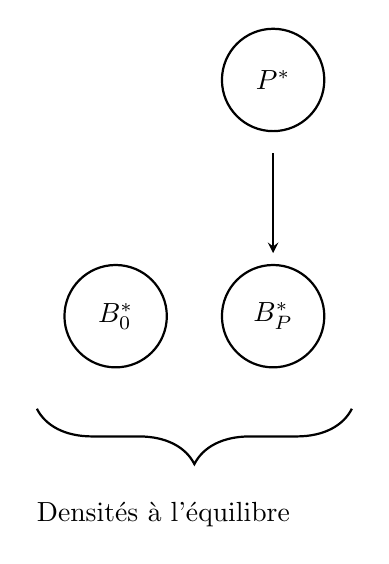
\begin{tikzpicture}[thick]
	\draw (6,3) circle (0.65);
	\node (P) at (6,3) {$P^*$};

	\draw (6,0) circle (0.65);
	\node (B) at (6,0) {$B^*_P$};

	\draw (4,0) circle (0.65);
	\node (B) at (4,0) {$B^*_0$};


	\node (PB) at (6,2.2) {};
	\draw[fleche] (PB) -- (6,0.8);



\draw[decoration={brace,mirror,raise=5pt,amplitude=20pt},decorate]
	  (3,-1) -- node[below=35pt, text width = 4cm] (D) {Densités à l'équilibre} (7,-1);

\end{tikzpicture}
% \end{figure}
%
% \end{document}
\par

\hfill\column{.5\textwidth}

\centering
Force nette d'interaction \[
\mathlarger{\dfrac{B^*_0}{B^*_P}}
\] \stopcols

\end{frame}

\begin{frame}{Stabilité du système}

\begincols
\column{0.48\textwidth}

\centering
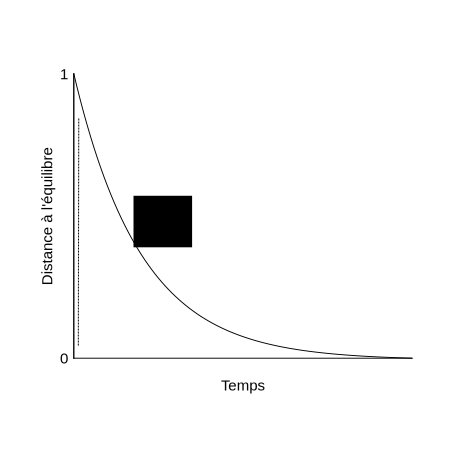
\includegraphics[width=1\linewidth]{figuresAz/disequ.pdf}

\hfill\column{0.48\textwidth}

\begin{itemize}
\tightlist
\item
  Perturbation ponctuelle: mortalité densité indépendante
\item
  Taux de retour: pente
\item
  Extinction
\end{itemize}

\stopcols

\end{frame}

\begin{frame}{Résultats attendus}

\begincols
 \column{.48\textwidth} \centering
Taux biologiques
\includegraphics[width=1.1\linewidth]{figuresAz/MTE.pdf} \pause
\column{.48\textwidth} \centering
Force nette d'interaction
\includegraphics[width=1.1\linewidth]{figuresAz/NetIS.pdf} \stopcols

\end{frame}

\begin{frame}{Résultats attendus}

\centering
Stabilité du système \par
\includegraphics[width=0.7\linewidth]{figuresAz/stabFinal.pdf}

\end{frame}

\begin{frame}{Approche quantitative: modélisation et expérimentations}

\begincols
 \column{.40\textwidth} \centering
 \input{figuresAz/schema_phd1.tex}\par
\column{.50\textwidth}
\includegraphics[width=1.2\linewidth]{figuresAz/yx.pdf} \stopcols

\end{frame}

\begin{frame}{Perspectives: Modèle multi-trophique}

\centering
% \documentclass[12pt,a4paper]{article}
%
% %%%%%%%%%%%%%%%%%%%%%%%%%%
% %% Packages %%
% % font
% \usepackage[T1]{fontenc}
% \usepackage[utf8]{inputenc}
% % language
% \usepackage[french, english]{babel}
%
% % marges, space...
% \usepackage[top=2.5cm, bottom=2.5cm, left=2.5cm, right=2.5cm]{geometry}
% \usepackage{setspace}
% \onehalfspacing
% \usepackage[font=footnotesize,labelfont=bf]{caption}
% \usepackage{subcaption}
%
% \usepackage{graphicx}
% \usepackage{float}
% \usepackage{pstool}
% \usepackage{multirow}
% \usepackage{booktabs,arydshln}
% % mathematics
% \usepackage{amsmath}
% \usepackage{textcomp}
%
% % TikZ
% \usepackage{tikz}
% 	\usetikzlibrary{arrows, plotmarks, decorations.markings}
% 	\tikzstyle{fleche} = [->,>=stealth,thick,rounded corners=4pt,line width=0.7pt]
% 	\tikzstyle{fleche2} = [->,>=stealth,thick,dashed,rounded corners=2pt,line width=0.5pt]
% 	\tikzstyle{trait} = [-,>=stealth,rounded corners=2pt,line width=0.7pt]
% 	\usetikzlibrary{shadows}
% 	\usetikzlibrary{shadings,decorations.pathreplacing,angles,quotes}
% 	\usetikzlibrary{positioning}
% %
% % %%%%%%%%%%%%%%%%%%%%%%%%%%
% %
%
% \begin{document}
%
%
% %% FIGURE MODEL %%
% \begin{figure}[!h]
% \centering
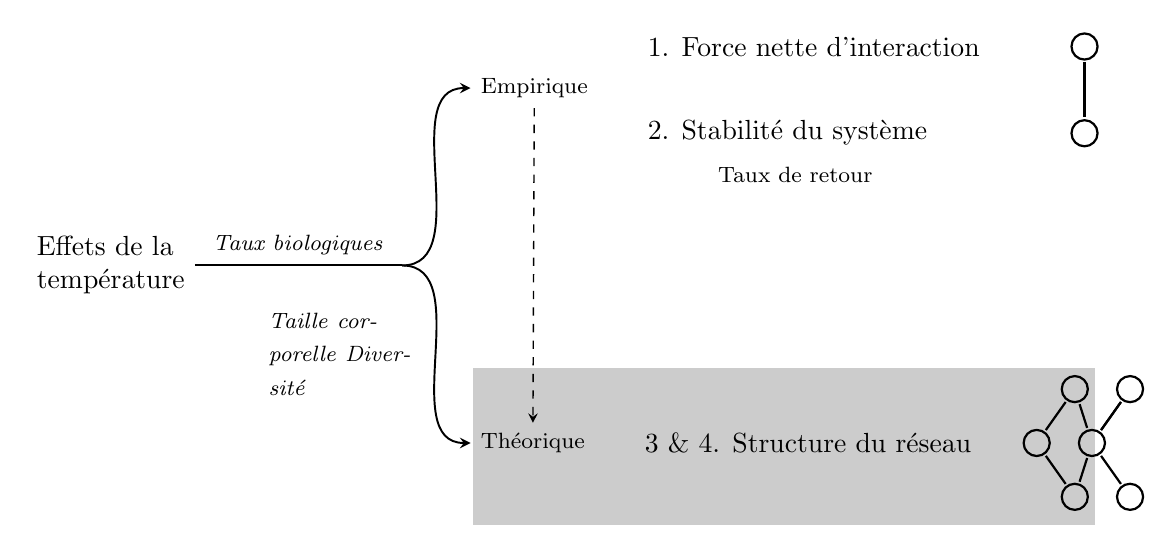
\begin{tikzpicture}[thick]

	\node (Titre) [align=left] at (3,4) {Effets de la \\ température};
	\node (FT) at (9,4){};

	\node [above right=1.5cm and 3.5cm of Titre](Emp) {\footnotesize{Empirique}};

	\node [below right=1.5cm and 3.5cm of Titre](Theo) {\footnotesize{Théorique}};

	\node [above right=0.02cm and 0.5cm of Emp](C1) {1. Force nette d'interaction};
	\node [below right=0.02cm and 0.5cm of Emp](C2) {2. Stabilité du système};
	\node [below=0.02cm of C2](stab) {\footnotesize{\hspace{0.1cm} Taux de retour}};

	\node [right=0.5cm of Theo](C3) {3 \& 4. Structure du réseau};
	%% Fleches


	\draw [fleche] (6.7,4) to [out=0,in=180] (Emp);
	\draw [fleche] (6.7,4) to [out=0,in=180] node[left, text width = 2cm] (Div) {\footnotesize{\textit{Taille corporelle Diversité}}}(Theo);

	\draw[trait] (Titre) -- (6.7,4) node [above, midway] {\footnotesize{\textit{Taux biologiques}}};

	\draw[fleche4] (Emp) -- (Theo) node [right] {};

	%% Réseau/Chaîne trophique

	\node[circle,draw,outer sep=1pt, right=1cm of C1] (c1) {};
	\node[circle,draw,outer sep=1pt, below=0.7cm of c1] (c2) {};
	\draw (c1) -- (c2);

	\node[circle,draw,outer sep=1pt, right=0.5cm of C3] (r1) {};
	\node[circle,draw,outer sep=1pt, right=0.3cm of r1] (r2) {};
	\node[circle,draw,outer sep=1pt, above right=0.4cm and 0.2cm of r1] (r3) {};
	\node[circle,draw,outer sep=1pt, right=0.3cm of r3] (r4) {};
	\node[circle,draw,outer sep=1pt, below right=0.4cm and 0.2cm of r1] (r5) {};
	\node[circle,draw,outer sep=1pt, right=0.3cm of r5] (r6) {};
	\draw (r5) -- (r1);
	\draw (r5) -- (r2);
	\draw (r1) -- (r3);
	\draw (r2) -- (r3);
	\draw (r2) -- (r4);
	\draw (r2) -- (r4);
	\draw (r6) -- (r2);

	\fill[black, opacity=0.2] (7.6,2.7) rectangle (15.5,0.7);


\end{tikzpicture}
%
% \end{figure}
%
% \end{document}
\par

\end{frame}

\begin{frame}{Merci de votre attention}

\centering
``An ecologist is often balancing the search for simplifying theories
with the recognition of the complexity of nature''

\hfill \textit{Charles Elton}

\end{frame}

\begin{frame}[plain]
  \begin{picture}(0,0)
    \put(-28.5,-175){%
      \pgfuseimage{titlebackground}
    }
  \end{picture}
\end{frame}

\end{document}
